\documentclass[11pt,a4paper]{article}
% ══════════════════════════════════════════════════════════════════════════════
% Edexcel Further Mathematics (Core Pure 1) --- Shared LaTeX Preamble
% Elegant, Minimalist & Aesthetic Academic Design System
% ══════════════════════════════════════════════════════════════════════════════

\usepackage[a4paper, top=22mm, bottom=22mm, left=20mm, right=20mm]{geometry}
\usepackage{amsmath, amssymb, amsthm}
\usepackage{enumitem}
\usepackage{booktabs}
\usepackage{array}
\usepackage{parskip}
\usepackage{microtype}
\usepackage{fancyhdr}
\usepackage{titlesec}
\usepackage{mdframed}
\usepackage{xcolor}
\usepackage[hidelinks]{hyperref}
\usepackage{graphicx}
\usepackage{tikz}
\usepackage{pgfplots}
\pgfplotsset{compat=1.18}

% ── Refined Palette ───────────────────────────────────────────────────────────
\definecolor{primary}{gray}{0.10}
\definecolor{darkgray}{gray}{0.20}
\definecolor{medgray}{gray}{0.50}
\definecolor{lightgray}{gray}{0.96}
\definecolor{boxgray}{gray}{0.85}
\definecolor{accentline}{gray}{0.75}

% ── Section formatting ──────────────────────────────────────────────────────────
\titleformat{\section}[block]
  {\normalfont\bfseries\color{primary}}{}
  {0pt}{}[\vspace{1pt}{\color{accentline}\rule{\textwidth}{0.4pt}}\vspace{4pt}]
\titlespacing*{\section}{0pt}{14pt}{6pt}

% ── List formatting ─────────────────────────────────────────────────────────────
\setlist[enumerate,1]{label=\textbf{\arabic*.}, leftmargin=1.8em, itemsep=14pt}
\setlist[enumerate,2]{label=\textbf{(\alph*)}, leftmargin=1.8em, itemsep=6pt}

% ── Header / footer (Overlaps permanently eliminated) ─────────────────────────
\pagestyle{fancy}
\newcommand{\CPHeader}[2]{%
  \fancyhf{}%
  \setlength{\headheight}{22pt}%
  \renewcommand{\headrulewidth}{0.3pt}%
  \renewcommand{\headrule}{\hbox to\headwidth{\color{accentline}\leaders\hrule height \headrulewidth\hfill}}%
  \fancyhead[L]{\footnotesize\scshape\color{medgray} Core Pure 1: #1}%
  \fancyhead[R]{\footnotesize\color{medgray} Chapter \##2}%
  \renewcommand{\footrulewidth}{0.3pt}%
  \renewcommand{\footrule}{\hbox to\headwidth{\color{accentline}\leaders\hrule height \footrulewidth\hfill}}%
  \fancyfoot[L]{\footnotesize\color{medgray} Pearson Edexcel A-Level Further Mathematics $\cdot$ Core Pure 1}%
  \fancyfoot[C]{}% No center text to ensure zero collision with long titles
  \fancyfoot[R]{\footnotesize\color{medgray} \textbf{Henry.K} \enspace$\vert$\enspace Page \thepage}%
}

% ── Elegant Aesthetic Title Block ──────────────────────────────────────────────
\newcommand{\CPTitleBlock}[2]{%
  \vspace*{-8pt}
  \begin{center}
    {\footnotesize\scshape\color{medgray} Pearson Edexcel A-Level Further Mathematics \enspace$\cdot$\enspace Core Pure 1}\\[4pt]
    {\LARGE\bfseries\color{primary} #1}\\[4pt]
    {\small\color{darkgray} #2}\\[6pt]
    {\footnotesize\color{medgray} Problem Series authored by \textbf{Henry.K} \quad$\cdot$\quad 10 Exam Archetypes \quad$\cdot$\quad 65 Total Marks}\\[8pt]
    {\color{accentline}\rule{\textwidth}{0.5pt}}
  \end{center}
  \vspace{-6pt}
  \noindent{\footnotesize\itshape \textbf{Instructions:} Answer all ten questions. Full algebraic working must be shown for method marks; unsupported answers from calculators will not gain full credit. Give exact values in surd or fractional form unless specified otherwise.}\par
  \vspace{3pt}
  {\color{accentline}\rule{\textwidth}{0.5pt}}
  \vspace{8pt}
}

% ── Answer / Method / Investigate-further boxes ────────────────────────────────
\newmdenv[
  backgroundcolor=lightgray,
  linecolor=boxgray,
  linewidth=0.5pt,
  roundcorner=3pt,
  leftmargin=0pt, rightmargin=0pt,
  innerleftmargin=10pt, innerrightmargin=10pt,
  innertopmargin=6pt, innerbottommargin=6pt,
  skipabove=5pt, skipbelow=5pt
]{ansbox}

\newmdenv[
  backgroundcolor=lightgray!40,
  linecolor=darkgray,
  linewidth=1.2pt,
  leftline=true, rightline=false, topline=false, bottomline=false,
  leftmargin=0pt, rightmargin=0pt,
  innerleftmargin=10pt, innerrightmargin=8pt,
  innertopmargin=5pt, innerbottommargin=5pt,
  skipabove=5pt, skipbelow=7pt
]{invbox}

\newcommand{\ans}[1]{%
  \begin{ansbox}
    \textbf{Answer:} #1
  \end{ansbox}}

\newcommand{\method}[1]{%
  {\small\textbf{Method Criteria:}\par\vspace{2pt}#1}\par}

\newcommand{\inv}[1]{%
  \begin{invbox}
    \textbf{\small Deep Investigation:} {\small #1}
  \end{invbox}}

\newcommand{\qn}[1]{\textbf{#1.}\;}

\usetikzlibrary{arrows.meta,calc}
\CPHeader{Linear Transformations}{7}

\begin{document}
\thispagestyle{plain}

\CPTitleBlock{Linear Transformations}{Problem Sheet \#7 \enspace$\cdot$\enspace 2D/3D Matrices, Invariant Lines, Area Scales \& Orientations}

\section*{Section A \quad Procedural \& Direct Foundations \hfill{\normalfont\footnotesize(Questions 1--3)}}
\begin{enumerate}
%── Q1 [DIR] ─────────────────────────────────────────────────────────────
\item \textbf{[DIR]} A rotation of $\frac{\pi}{3}$ radians anticlockwise about the origin is represented by the matrix $\mathbf{R}$.
\begin{enumerate}
  \item Write down the matrix $\mathbf{R}$, giving entries in exact form. \hfill{\small\textbf{[2]}}
  \item Find the image of the point $P(2, 0)$ under $\mathbf{R}$. \hfill{\small\textbf{[1]}}
  \item Reflection in the line $y = x\tan\frac{\pi}{6}$ is represented by the matrix $\mathbf{S}$. Write down $\mathbf{S}$, giving entries in exact form. \hfill{\small\textbf{[2]}}
\end{enumerate}

%── Q2 [DIR] ─────────────────────────────────────────────────────────────
\item \textbf{[DIR]} A shear with the $x$-axis invariant maps the point $(0, 1)$ to the point $(3, 1)$.
\begin{enumerate}
  \item Write down the $2 \times 2$ matrix $\mathbf{H}$ representing this shear. \hfill{\small\textbf{[2]}}
  \item The enlargement with centre the origin and scale factor $2$ is represented by matrix $\mathbf{E}$. Find the matrices $\mathbf{E}\mathbf{H}$ and $\mathbf{H}\mathbf{E}$. \hfill{\small\textbf{[3]}}
  \item Explain why $\mathbf{E}\mathbf{H} = \mathbf{H}\mathbf{E}$ in this case, and state when two $2 \times 2$ matrices always commute. \hfill{\small\textbf{[1]}}
\end{enumerate}

%── Q3 [DIR] ─────────────────────────────────────────────────────────────
\item \textbf{[DIR]} The triangle $T$ has vertices $A(1, 0)$, $B(0, 1)$, and $C(1, 1)$. The linear transformation $\mathbf{M}$ is given by
\[
\mathbf{M} = \begin{pmatrix} 2 & 1 \\ 1 & 3 \end{pmatrix}
\]
\begin{enumerate}
  \item Find the coordinates of $A'$, $B'$, $C'$, the images of $A$, $B$, $C$ under $\mathbf{M}$. \hfill{\small\textbf{[2]}}
  \item Calculate the area of triangle $T$. \hfill{\small\textbf{[1]}}
  \item Calculate the area of triangle $T'$ and verify that $\frac{\text{Area}(T')}{\text{Area}(T)} = |\det(\mathbf{M})|$. \hfill{\small\textbf{[3]}}
\end{enumerate}

\begin{center}
\begin{tikzpicture}[scale=1.1, >=Stealth]
  % Axes
  \draw[->, gray!60] (-0.5,0) -- (5.5,0) node[right] {\footnotesize $x$};
  \draw[->, gray!60] (0,-0.5) -- (0,4.5) node[above] {\footnotesize $y$};

  % Original triangle T (blue)
  \fill[blue!20, opacity=0.6] (1,0) -- (0,1) -- (1,1) -- cycle;
  \draw[blue!70!black, thick] (1,0) -- (0,1) -- (1,1) -- cycle;
  \node[blue!70!black, font=\footnotesize, below] at (1,0) {$A(1,0)$};
  \node[blue!70!black, font=\footnotesize, left] at (0,1) {$B(0,1)$};
  \node[blue!70!black, font=\footnotesize, above left] at (1,1) {$C(1,1)$};
  \node[blue!70!black, font=\scriptsize\bfseries] at (0.6,0.55) {$T$};

  % Image triangle T' (red): A'=(2,1), B'=(1,3), C'=(3,4)
  \fill[red!20, opacity=0.5] (2,1) -- (1,3) -- (3,4) -- cycle;
  \draw[red!70!black, thick] (2,1) -- (1,3) -- (3,4) -- cycle;
  \node[red!70!black, font=\footnotesize, below right] at (2,1) {$A'(2,1)$};
  \node[red!70!black, font=\footnotesize, left] at (1,3) {$B'(1,3)$};
  \node[red!70!black, font=\footnotesize, right] at (3,4) {$C'(3,4)$};
  \node[red!70!black, font=\scriptsize\bfseries] at (2,2.5) {$T'$};

  % Mapping arrows
  \draw[->, densely dashed, gray!70] (1,0.1) to[bend left=20] (1.9,0.9);
  \draw[->, densely dashed, gray!70] (0.1,1.1) to[bend left=15] (0.9,2.8);
  \draw[->, densely dashed, gray!70] (1.1,1.15) to[bend left=15] (2.8,3.8);

  \node[font=\scriptsize\itshape, text=medgray, align=center] at (2.8,-0.7) {Figure 7.1: Triangle $T$ and its image $T'$ under $\mathbf{M}$};
\end{tikzpicture}
\end{center}

\end{enumerate}

\section*{Section B \quad Reverse Parameters \& Analysis \hfill{\normalfont\small(Questions 4--6)}}
\begin{enumerate}[resume]
%── Q4 [REV] ─────────────────────────────────────────────────────────────
\item \textbf{[REV]} The matrix $\mathbf{M} = \begin{pmatrix} 3 & -1 \\ 2 & 4 \end{pmatrix}$ represents a linear transformation.
\begin{enumerate}
  \item Find $\det(\mathbf{M})$ and state the area scale factor. \hfill{\small\textbf{[2]}}
  \item Determine whether $\mathbf{M}$ preserves or reverses orientation. \hfill{\small\textbf{[1]}}
  \item The unit square $S$ has vertices $(0,0)$, $(1,0)$, $(1,1)$, $(0,1)$. Find the vertices of the image of $S$ under $\mathbf{M}$ and verify that the image has area $|\det(\mathbf{M})|$. \hfill{\small\textbf{[3]}}
\end{enumerate}

%── Q5 [REV] ─────────────────────────────────────────────────────────────
\item \textbf{[REV]} The transformation $T$ is represented by $\mathbf{M} = \begin{pmatrix} 5 & 4 \\ 4 & 5 \end{pmatrix}$.
\begin{enumerate}
  \item Find all invariant points of $T$, i.e.\ all points $\begin{pmatrix} x \\ y \end{pmatrix}$ such that $\mathbf{M}\begin{pmatrix} x \\ y \end{pmatrix} = \begin{pmatrix} x \\ y \end{pmatrix}$. \hfill{\small\textbf{[3]}}
  \item Find all lines of invariant points of $T$ (lines on which \emph{every} point maps to itself). \hfill{\small\textbf{[3]}}
\end{enumerate}

%── Q6 [REV] ─────────────────────────────────────────────────────────────
\item \textbf{[REV]} Reflection in the line $y = x$ is represented by the matrix $\mathbf{M} = \begin{pmatrix} 0 & 1 \\ 1 & 0 \end{pmatrix}$.
\begin{enumerate}
  \item Find all lines of invariant points. \hfill{\small\textbf{[2]}}
  \item Find all invariant lines through the origin (lines that map to themselves, but where individual points may move). \hfill{\small\textbf{[3]}}
  \item On a diagram, show the invariant line, the line of invariant points, and illustrate how the point $(3, 1)$ maps to $(1, 3)$. \hfill{\small\textbf{[1]}}
\end{enumerate}

\begin{center}
\begin{tikzpicture}[scale=0.75, >=Stealth]
  % Axes
  \draw[->, gray!60] (-0.5,0) -- (5,0) node[right] {\footnotesize $x$};
  \draw[->, gray!60] (0,-0.5) -- (0,5) node[above] {\footnotesize $y$};

  % Line y = x (line of invariant points)
  \draw[thick, blue!70!black] (-0.3,-0.3) -- (4.5,4.5);
  \node[blue!70!black, font=\footnotesize, rotate=45] at (3.8,4.2) {$y = x$};

  % Line y = -x (invariant line)
  \draw[thick, red!70!black, dashed] (-0.3,0.3) -- (3.5,-3.5+4.5);

  % Points (3,1) and (1,3)
  \filldraw[black] (3,1) circle (2pt) node[below right, font=\footnotesize] {$(3,1)$};
  \filldraw[black] (1,3) circle (2pt) node[above left, font=\footnotesize] {$(1,3)$};
  \draw[->, thick, orange!80!black] (2.9,1.1) -- (1.1,2.9);

  % Perpendicular bisector marker on y=x at (2,2)
  \filldraw[blue!70!black] (2,2) circle (1.5pt);
  \node[blue!70!black, font=\scriptsize, right] at (2.1,2.1) {$(2,2)$};

  \node[font=\scriptsize\itshape, text=medgray, align=center] at (2.5,-0.7) {Figure 7.2: Reflection in $y=x$ mapping $(3,1) \mapsto (1,3)$};
\end{tikzpicture}
\end{center}

\end{enumerate}

\newpage
\section*{Section C \quad Proof, Geometry \& Multi-step \hfill{\normalfont\small(Questions 7--10)}}
\begin{enumerate}[resume]
%── Q7 [REV] ─────────────────────────────────────────────────────────────
\item \textbf{[REV]} The matrix $\mathbf{M} = \begin{pmatrix} 3 & 1 \\ 0 & 2 \end{pmatrix}$ represents a linear transformation.
\begin{enumerate}
  \item Show that the only invariant point is the origin. \hfill{\small\textbf{[2]}}
  \item Find all invariant lines of the form $y = mx + c$ that pass through the origin. \hfill{\small\textbf{[3]}}
  \item Find all invariant lines of the form $y = mx + c$ that do \emph{not} pass through the origin. \hfill{\small\textbf{[3]}}
\end{enumerate}

%── Q8 [GEO] ─────────────────────────────────────────────────────────────
\item \textbf{[GEO]} The reflection in the $xy$-plane ($z = 0$) is represented by the $3 \times 3$ matrix $\mathbf{R}$.
\begin{enumerate}
  \item Write down $\mathbf{R}$. \hfill{\small\textbf{[1]}}
  \item The point $P$ has position vector $\begin{pmatrix} 3 \\ -1 \\ 4 \end{pmatrix}$. Find the image $P'$ of $P$ under $\mathbf{R}$. \hfill{\small\textbf{[1]}}
  \item Let $\mathbf{Q}$ represent reflection in the $xz$-plane ($y = 0$). Write down $\mathbf{Q}$ and find the composite matrix $\mathbf{Q}\mathbf{R}$. \hfill{\small\textbf{[2]}}
  \item Describe geometrically the single transformation represented by $\mathbf{Q}\mathbf{R}$. \hfill{\small\textbf{[2]}}
\end{enumerate}

\begin{center}
\begin{tikzpicture}[scale=0.85, >=Stealth, z={(0.35cm,0.25cm)}]
  % Axes
  \draw[->, gray!60] (0,0,0) -- (4.5,0,0) node[right] {\footnotesize $x$};
  \draw[->, gray!60] (0,0,0) -- (0,3.5,0) node[above] {\footnotesize $z$};
  \draw[->, gray!60] (0,0,0) -- (0,0,5) node[below left] {\footnotesize $y$};

  % xy-plane (shaded)
  \fill[blue!8, opacity=0.5] (0,0,0) -- (4,0,0) -- (4,0,4) -- (0,0,4) -- cycle;
  \draw[blue!40, thin] (0,0,0) -- (4,0,0) -- (4,0,4) -- (0,0,4) -- cycle;
  \node[blue!60!black, font=\scriptsize] at (2.5,0,3.5) {$z = 0$ plane};

  % Point P
  \filldraw[red!70!black] (3,3.2,-1) circle (2pt);
  \node[red!70!black, font=\footnotesize, above right] at (3,3.2,-1) {$P(3,-1,4)$};

  % Point P'
  \filldraw[teal!70!black] (3,-3.2,-1) circle (2pt);
  \node[teal!70!black, font=\footnotesize, below right] at (3,-3.2,-1) {$P'(3,-1,-4)$};

  % Dashed connection through mirror plane
  \draw[dashed, gray!70] (3,3.2,-1) -- (3,-3.2,-1);

  % Tick marks at midpoint
  \filldraw[gray] (3,0,-1) circle (1pt);

  \node[font=\scriptsize\itshape, text=medgray, align=center] at (2.5,-2.5,0) {Figure 7.3: Reflection of $P$ in the $xy$-plane};
\end{tikzpicture}
\end{center}

%── Q9 [GEO] ─────────────────────────────────────────────────────────────
\item \textbf{[GEO]} The $3 \times 3$ matrix $\mathbf{R}_z(\theta)$ represents a rotation of angle $\theta$ anticlockwise about the $z$-axis (when viewed from above).
\begin{enumerate}
  \item Write down $\mathbf{R}_z\!\left(\frac{\pi}{2}\right)$. \hfill{\small\textbf{[2]}}
  \item Find the image of the point $(1, 0, 2)$ under $\mathbf{R}_z\!\left(\frac{\pi}{2}\right)$. \hfill{\small\textbf{[1]}}
  \item The $3 \times 3$ matrix $\mathbf{R}_x\!\left(\frac{\pi}{2}\right)$ represents a rotation of $\frac{\pi}{2}$ anticlockwise about the $x$-axis. Write down $\mathbf{R}_x\!\left(\frac{\pi}{2}\right)$. \hfill{\small\textbf{[2]}}
  \item Find the matrix $\mathbf{C} = \mathbf{R}_x\!\left(\frac{\pi}{2}\right) \, \mathbf{R}_z\!\left(\frac{\pi}{2}\right)$ and verify that $|\det(\mathbf{C})| = 1$. \hfill{\small\textbf{[3]}}
\end{enumerate}

%── Q10 [SYN] ─────────────────────────────────────────────────────────────
\item \textbf{[SYN]} A linear transformation in $\mathbb{R}^3$ is represented by the matrix
\[
\mathbf{M} = \begin{pmatrix} 2 & 0 & 0 \\ 0 & 3 & 0 \\ 0 & 0 & 1 \end{pmatrix}
\]
\begin{enumerate}
  \item Find $\det(\mathbf{M})$ and state the volume scale factor of $\mathbf{M}$. \hfill{\small\textbf{[2]}}
  \item A unit cube with one vertex at the origin is mapped under $\mathbf{M}$. Describe the image and find its volume. \hfill{\small\textbf{[2]}}
  \item The matrix $\mathbf{N} = \mathbf{R}_z\!\left(\frac{\pi}{2}\right)$ from Question~9 represents a rotation about the $z$-axis. Find $\mathbf{N}\mathbf{M}$ and determine $\det(\mathbf{N}\mathbf{M})$. \hfill{\small\textbf{[3]}}
  \item Explain why the volume scale factor is unchanged by the rotation. \hfill{\small\textbf{[1]}}
\end{enumerate}

\end{enumerate}

\vspace{10pt}
\begin{center}
  {\color{accentline}\rule{0.4\textwidth}{0.4pt}}\\[4pt]
  {\footnotesize\itshape\color{medgray} ``Symmetry, as wide or narrow as you may define its meaning, is one idea by which man through the ages has tried to comprehend and create order, beauty, and perfection.''}\\[2pt]
  {\scriptsize\scshape\color{medgray} Hermann Weyl}\\[4pt]
  {\color{accentline}\rule{0.4\textwidth}{0.4pt}}
\end{center}

\end{document}
